% Supplemental direction tips on the user's unchanged vector drawing.
% Coordinates are PDF points from the panel's upper-left corner.
\documentclass[border=0pt]{standalone}
\usepackage{graphicx,tikz}
\usetikzlibrary{arrows.meta}
\definecolor{acol}{RGB}{245,154,35}
\definecolor{dcol}{RGB}{130,33,139}
\begin{document}%
\begin{tikzpicture}[x=1bp,y=-1bp,
  tip/.style={line width=.55bp,-{Stealth[length=3.7bp,width=2.7bp]},line cap=round},
  atip/.style={tip,acol},dtip/.style={tip,dcol}]
\path[use as bounding box] (0,0) rectangle (216,328);
\begin{scope}[overlay]
\node[anchor=north west,inner sep=0pt,outer sep=0pt] at (0,0)
  {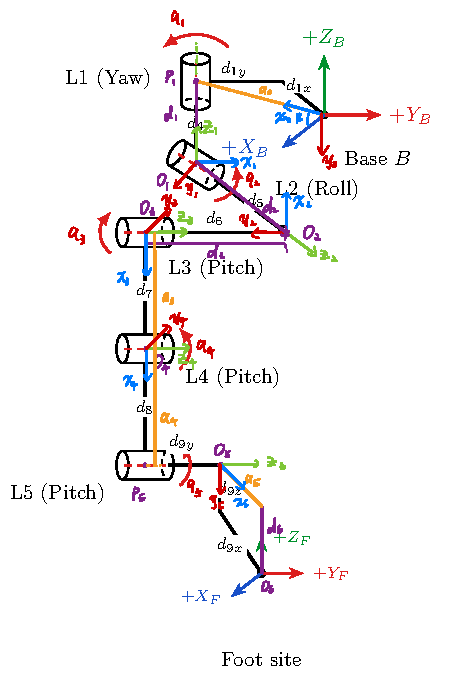
\includegraphics[width=216bp,height=328bp]{../assets/dh_right_handdrawn.pdf}};
% a_0: base to the yaw-axis intermediate point, upper-left.
\draw[atip] (102.0,41.0)--(94.2,39.0);
% d_1: yaw-axis intermediate point to the roll-axis origin, downward.
\draw[dtip] (94.1,71.2)--(94.1,77.6);
% d_2: roll-axis origin to pitch-axis intermediate point, lower-right.
\draw[dtip] (131.7,107.0)--(137.7,111.7);
% d_3: the existing offset purple dimension line, right to left.
\draw[dtip] (78.4,117.1)--(70.4,117.1);
% a_3 and a_4: the existing orange vertical dimension segments.
\draw[atip] (74.4,159.0)--(74.4,166.9);
\draw[atip] (74.4,215.3)--(74.4,223.2);
% d_5: missing purple segment; the black rigid-link edge remains visible.
\draw[dtip,line width=.4bp] (69.5,223.4)--(104.7,223.1);
\node[dcol,font=\fontsize{6}{6}\selectfont,inner sep=0pt] at (95.2,219.0) {$d_5$};
% a_5: the existing orange ankle-to-site transverse component.
\draw[atip] (119.8,237.3)--(125.4,242.9);
% d_6: the existing purple component into the foot site.
\draw[dtip] (125.7,267.4)--(125.7,274.9);
\end{scope}
\end{tikzpicture}%
\end{document}
